\documentclass[9pt,twocolumn,twoside]{pnas-new}

% Use the lineno option to display guide line numbers if required.
% Note that the use of elements such as single-column equations
% may affect the guide line number alignment. 
\templatetype{pnasresearcharticle} 

% Choose template 
% {pnasresearcharticle} = Template for a two-column research article
% {pnasmathematics} = Template for a one-column mathematics article
% {pnasinvited} = Template for a PNAS invited submission
\usepackage{amsthm} 
\usepackage{amsmath} 
\usepackage{amssymb} 
\usepackage{multicol} 
\usepackage{array}
\usepackage{hyperref}

\DeclareMathOperator*{\argmax}{argmax} 
\newtheorem{axiom}{Axiom} 
\newtheorem{theorem}{Theorem}

% \title{Curiosity is an optimal solution to the exploration-exploitation dilemma}
\title{A way around the exploration-exploitation dilemma.}

\author[a,b,1]{Erik J Peterson} 
\author[a,b,c,d]{Timothy D Verstynen} 
\affil[a]{Department of Psychology} 
\affil[b]{Center for the Neural Basis of Cognition} 
\affil[c]{Carnegie Mellon Neuroscience Institute}
\affil[d]{Biomedical Engineering, Carnegie Mellon University, Pittsburgh PA}
\leadauthor{Peterson} 
\authordeclaration{The authors have no conflicts of interest to declare.}

% \equalauthors{\textsuperscript{1}A.O.(Author One) and A.T. (Author Two) contributed equally to this work (remove if not applicable).}
\correspondingauthor{\textsuperscript{1}To whom correspondence should be addressed. E-mail: Erik.Exists@gmail.com}

\begin{abstract}
For all animals the decision to explore comes with a risk of getting less. For example, a foraging bee might find less nectar, or hunting hawk less prey. This loss is often formalized as regret. It's been mathematically proven that exploring an uncertain world with a specific goal always has some regret. This is why exploration-exploitation can be a dilemma. Given this proof we wondered if the common advice to ``focus on learning and not the goal'' might have mathematical merit. So we re-imagined exploration in the dilemma as an open ended search for any new information. We then developed a new minimal description of information value, which generalizes existing ideas like curiosity, novelty and information gain. We use this description to model the dilemma as a competition between strategies that maximize reward and information independently. Here we prove this competition has a no regret solution. When we study this solution in simulation -- using classic bandit tasks -- it outperforms standard approaches, especially when rewards are sparse.
\end{abstract}

% SIGNIFICANCE
\significancestatement{
The uncertainty of the unknown can always be recast as an opportunity to learn. But learning doesn't look like enough compensation when, for example, you're a bee foraging for nectar or a hawk hunting for prey. An animal exploring though quickly finds itself with a difficult question. Is it better to keep exploring, or stick with the known? This problem, the exploration-exploitation dilemma, is mathematically intractable. 

When one mathematical problem can’t be solved perfectly, it’s often good to find another related problem that can be. In this work we show that when exploration is re-imagined as an open-ended search to learn as much as possible, it actually becomes possible to solve exploration-exploitation optimally. Perhaps learning is enough, after all.
}
% \dates{This manuscript was compiled on \today}
% \doi{\url{www.pnas.org/cgi/doi/10.1073/pnas.XXXXXXXXXX}}
\begin{document} 
\verticaladjustment{-2pt} 
\maketitle

\thispagestyle{firststyle} \ifthenelse{\boolean{shortarticle}}{\ifthenelse{\boolean{singlecolumn}}{\abscontentformatted}{\abscontent}}{}

% TODO: the search for reward depends on having a good world model. This is not made clear. Such limits are not discussed... enough? Fix this during revision!
\section*{Introduction}
Decision making in the natural world often leads to a dilemma. As an example let's imagine a bee foraging in a meadow (Figure~\ref{fig:f1}\textbf{A}). The bee could go to the location of a flower it's been to before to gather nectar. Or the bee go somewhere new, and explore. Exploration comes though with the risk of getting less nectar. Perfectly optimizing away this risk is a mathematically intractable problem; there is no way to explore without enduring some regret \cite{Thrun1992a,Dayan1996,Findling2018,Gershman2018b}, and so the decision can become a dilemma.

Resource gathering is not the only reason animals explore. Many animals, like our bee, explore out of curiosity (Figure~\ref{fig:f1}\textbf{B}). This exploration lets them learn about their environment, developing an often simplified model that helps them in planning actions and making future decisions \cite{Ahilan2019,Poucet1993}. Borrowing from the field of artificial intelligence we refer to these models as \textit{world models} \cite{`Schmidhuber2019,Sutton2018,Schmidhuber1991'}. World models offer a principled explanation for why animals are intrinsically curious \cite{Mehlhorn2015,Gupta2006,Berger-Tal2014,Gottlieb2018,Schwartenbeck2019,Pathak2017}, and prone to explore even when no rewards are present or expected \cite{Hughes1997}. 

Curiosity raises the question of whether animals need to explore looking for specific goals or rewards are all. Perhaps we've misinterpreted their actions, and so misconceived of a fundamental problem in the learning and decision sciences. Here we explore a bold conjecture:

\begin{quote}
`Exploration for reward is never needed. The only exploratory behavior an animal needs is that which builds its world model. '   
\end{quote}

\begin{figure}
	[tbhp] \centering 
	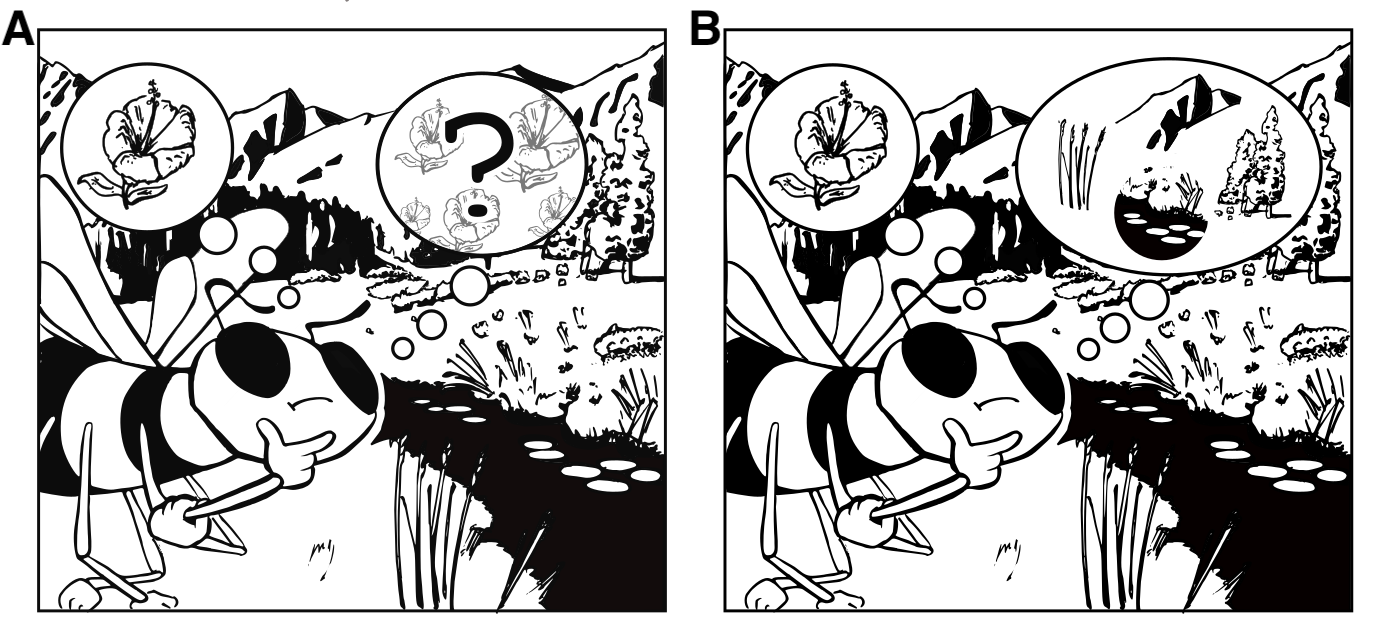
\includegraphics[width=.95\linewidth]{figures/fig1.png} 
	\caption{Two views of exploration and exploitation. \textbf{A}. The classic dilemma: either exploit an action with a known reward (e.g., return to the previous plant) or explore other actions on the chance they will return a better outcome (e.g., find a plant with more flowers). \textbf{B.} Here we offer an alternative view of the dilemma, with two different competitive goals: maximize rewards (e.g., keep returning to known flower locations) \texti{or} build a world model by learning new information (e.g., layout of the environment). Exploration here focused on learning in general, not on reward learning specifically. \textit{Artist credit}: Richard Grant.}
	\label{fig:f1} 
\end{figure}

Our contribution is threefold. We define a new minimal (axiomatic) description for information value, which generalizes existing ideas like curiosity, novelty and information gain. In fact, the axioms let us formally disconnect information theory \cite{Shannon1948} from information value, suggesting we may have uncovered a new universal theory. Next we prove that the computer science method of dynamic programming \cite{Bellmann1954,Sutton2018} provides an optimal way to maximize this kind of information value. Finally, we describe a simple winner-take-all scheduling algorithm that can optimally solve a competition between strategies which independently maximize information value and reward. 

\section*{Results}
Tangible rewards are a conserved resource, but learned information isn't. For example, if a rat shares potato chip with a cage-mate, she must necessarily split up the chip leaving less food for herself. Whereas if student shares the latest result from a scientific paper with a lab-mate, they do not necessarily forget a portion of that result. These differences  make reward and information different concepts, and so considering information as a kind of reward isn't consistent.  

If information value isn't a reward, we need another way to study and value it. To do this we first looked to the field of information theory \cite{Shannon1948}, but the problem of information value is not based in the statistical problem of transmitting symbols, as was Shannon’s goal. It is based on the problem of learning and remembering them.

\subsection*{A minimal model of memory}
World models are memories with some amount of simplification \cite{Schmidhuber1991,Ha2018}. They can range from simple novelty signals \cite{Kakade2002}, to location or state counts \cite{Bellemare2016,Dayan1993}, state and action prediction \cite{Schmidhuber1991,Pathak2017,Friston2016}, flow \cite{Yang2019}, learning progress \cite{Lopes2012}, classic working or episodic memories \cite{Miller1956,Tulving2002}, Bayesian and hierarchical Bayesian models \cite{Park2017,Itti2009,Friston2016,Tenenbaum2006}, latent spaces \cite{Kingma2013} and recurrent neural networks \cite{Ganguli2008,Ha2018,Schmidhuber2015a,Mante2013}. 

We have no mathematical reason to prefer any one kind of world model over any other. So we designed a new minimal definition, designed to overlap with all of them.

We must introduce some intial notation. We assume that time is a continuous value and denote increases in time using the differential quantity $dt$. We can then express changes in $M$ (our world model, defined below) as a gradient, $\nabla M$. We also assume that observations about the environment $s$ are real numbers sampled from a finite state space $s \in S$, whose size is $N$ (denoted $S^N$). Actions are also real numbers $a$, drawn from a finite space $A^K$. Rewards $R_t$ -- when they appear -- are binary $(0,1)$ and are provided \textit{only} by the external environment. 

\textit{Definition 1.} We can now formally define a world model $M$ as a finite set of real numbers, whose maximum size is $L$ ($M^L$). We say that every world model has a pair of functions $f$ and $g$. Learning of $s$ at time $t$ (i.e. $s_t$) by $M$ is done by the invertible encoder function $f$, $M_{t+dt} = f(M_{t}, s_{t})$ and $M_{t} = f^{-1}(M_{t+dt}, s_{t})$. Memories $\hat s_t$ about $s_t$ are recalled by the decoder function $g$, $\hat s_t = g(M_t, s_t)$. 

The invertibility of $f$, denoted as $f^{-1}$, is a mathematical way to ensure that any observations encoded in the world model can also be forgotten. This is both an important aspect of real memory, and a critical point for our mathematical analysis.

The details of $f$ and $g$ define what kind of world model or memory $M$ is. Let's consider some examples. If $f$ adds states $s_t$ to the memory, and $g$ tests whether $s_t$ is in $M$, then $M$ is a model of novelty \cite{Kakade2002}. If $f$ counts states and $g$ returns those counts, then $M$ is a count-based heuristic \cite{Bellemare2016,Dayan1993}. If $f$ follows Bayes rule and $g$ decodes the probability of $s_t$, then $M$ is a Bayesian memory \cite{Itti2009,Friston2016,Tenenbaum2006,Schmidhuber1991,Pathak2017,Friston2016}. If the size of $M$ is much smaller than the size of the state space $S^N$, then $f$ can be seen as learning a latent or compressed representation im $M$ \cite{Kingma2013,Schmidhuber2008,Levi-Aharoni2019,Ganguli2010,Ha2018,Schmidhuber2015a,Mante2013,Park2017}, and $g$ decodes a reconstruction of $s$ ($\hat s_t$) or future states ($\hat s_{t+dt}$).
 
% \subsubsection*{Axioms for information value}
% In all of these examples, the value of any observation made by an agent who is learning a world model depends entirely on what the agent learns by making that observation.
% \begin{axiom}
% 	[Axiom of Memory] The value of $E(s_t)$ depends \emph{only} on how the memory $M$ changes.
% \label{ax:1} \end{axiom}
% \noindent This axiom does two things. It ensures value depends only on the memory, and how it changes. And in particular it ensures value depends only on the most recent change in $M$. That driven by observing $s_t$. Readers familiar with reinforcement learning can see this as a natural way to induce the Markov property on the memory.
% \begin{axiom}
% 	[Axiom of Novelty] The value of $E(s_t)$ is zero only when $\nabla M$ is zero. 
% \label{ax:2} \end{axiom}
% \begin{axiom}
% 	[Axiom of Scholarship] Learning can't lead to negative value, so the value of $E(s_t) \geq 0$.
% \label{ax:3} \end{axiom}
% \begin{axiom}
%     [Axiom of Maximum Difference] The value of $E(s_t)$ should be the maximum value which depends on the total change in $M$.
% \label{ax:4} \end{axiom}

% \begin{axiom}
%     [Axiom of Specificity] If the total change in memory $M$ due to observation $s_t$ is held constant ($\frac{dM}{dt} = h$), the more compact (Eq.~\ref{eq:compactcude}) the change in memory the more valuable the observation. 
% \label{ax:4} \end{axiom}
% \noindent Axiom~\ref{ax:4} adds two critical and intertwined properties. It ensures that if all else is held equal, more specific observations are more valuable that less specific observations \cite{Berlyne1950,Kidd2015}. It also ensures that an observation that leads to a simplifying or parsimonious insight (is equivalent to a compression of the memory, \cite{Schmidhuber2008}) is more valuable than one that changes memory the same total amount but does not lead to compression.

% TODO: this can be violated easily. Visit the full def of PAC learning
% and just use that... skip NP?
% \begin{axiom}
% 	[Axiom of Equilibrium] An observation $s_t$ must be learnable by $M$. $\frac{d^2M(s_t)}{dt^2} \leq 0$. 
% \label{ax:5} \end{axiom}

% TODO: this whole section needs a re-write based on the slides
\subsection*{A minimal description of information value.}
To formalize information value we use two axioms that define a real valued function, $E(s)$, that measures the value of any observation $s_t$ given a world model $M$ and a distance metric $d$.

\begin{axiom}
    [Axiom of Change] The value of information $E(s_t)$ depends only on the total distance $M$ moves by making observation $s_t$.
\label{ax:4} \end{axiom}

\noindent This axiom does three important things. It ensures information value depends only on the world model, that value is a distance in memory, and that value learning has the Markov property \cite{Sutton2018}. Now, let's unpack it.

By distance we mean a function $\delta = d(m,m')$, where $m \in M$ and $m' \in M'$ are discrete memories drawn from two memories $M$ and $M'$. We define $d$ so $d \ge 0$ for all $s \in S$, and let $d = 0$ only if $M = M'$. Our definition of $d$ \textit{does not} require the distance in memories from $M$ to $M'$ be the same as from $M'$ to $M$. Nor for the triangle inequality to hold. For the technically inclined, this definition makes $d$ a pre-metric. 

By total distance we mean the norm $||\Delta||$, where $\Delta = \{\delta_1, \delta_2,...,\delta_L\}$. 

In summary, Let $E \equiv ||\Delta||$.

Different $f$ and $g$ pairs will naturally need different ways to measure distances in $M$. For example, in a novelty world model \cite{Kakade2002} either the hamming or Manhattan distance are applicable and would produce binary distance values, as would a count model \cite{Bellemare2016,Dayan1993}. A latent memory \cite{Schmidhuber1991,Pathak2017} might instead use the euclidean norm of its own error gradient \cite{Pascanu2013}. While a probabilistic or Bayesian memory would likely use the Kullback–Leibler (KL) divergence \cite{Park2017,Friston2016}.
 
\begin{axiom}
	[Axiom of Equilibrium] To be valuable an observation $s_t$ must be learnable by $M$ 
\label{ax:5} 
\end{axiom}

\noindent By learnable we mean two things. First, with every (re)observation of $s$, $M$ should change. Second, the change in $M$ must eventually reach a learned equilibrium. To formalize these we constrain the average gradient of $M$, so $\mathbb{E}\big [\nabla^2 M \big ] \leq 0$. 

Most attempts to value information rest their definition on information theory. Value might rest on the intrinsic complexity of an observation (i.e., its entropy) \cite{Haarnoja2018} or on its similarity to the environment (i.e., mutual information) \cite{Kolchinsky2018}, or on some other salience signal \cite{Tishby2000}. In our analysis, learning alone drives value. This is because learning might happen on a true world model or with a faulty world model, or be about a fictional narrative. The observation might be simple, or complex. From a subjective point of view, which is the right point of view for value, all of these are the same; value depends only on the total knowledge gained.

\subsection*{Exploration as a dynamic programming problem} Dynamic programming is a popular optimization method because it guarantees value is maximized using a simple algorithm that always chooses the largest option. In Theorem~\ref{theorem:opt_sub} (see \textit{Mathematical Appendix}) we prove that our definition of memory has one critical property, optimal substructure, that is needed for an optimal dynamic programming solution \cite{Bellmann1954,Roughgarden2019}. The other two required properties, $E \ge 0$ and the Markov property \cite{Bellmann1954,Roughgarden2019}, are fulfilled by the \textit{Axiom 1}. 
To write down our dynamic programming solution we introduce a little more notation. We let $\pi$ denote an action policy, a function that takes a state $s$ and returns an action $a$. We let $\delta$ denote the transition function, which takes a state-action pair $(s_{t},a_t)$ and returns a new state, $s_{t+dt}$. This function acts as an abstraction for the actual world. For notational consistency with the standard Bellman approach we also redefine $E(s)$ as a \textit{payoff function}, $F(M_{t}, a_t)$ \cite{Bellmann1954}.
 
\begin{equation}
	\begin{split}\label{eq:payout} 
		F(M_{t}, a_t) = E(s)\\
		\text{subject to the constraints} \\
		a_{t} = \pi(s_t) \\
		s_{t+dt} = \delta(s_{t}, a_t),\\
		M_{t+dt} = f(M_{t}, s_{t}) 
	\end{split}
\end{equation}

\noindent The value function for $F$ is,

\begin{equation}\label{eq:V_E} 
	\begin{split}
		V_{\pi_E}(M_0) = \Big [ \max_{a \in A} \sum_{t=0}^{\infty} F(M_t, a_t) \ \Big | \ M, \ d, \ S \ \Big ]. 
	\end{split}
\end{equation}

\noindent And the recursive Bellman solution to learn this value function is,

\begin{equation}\label{eq:bellman_iter} 
	V^*_{\pi_E}(M_{t}) = F(M_{t}, a_{t}) + \max_{a \in A} \Big [ F(M_{t+dt}, a_t) \Big ].
\end{equation}

For the full derivation of Eq~\ref{eq:bellman_iter} see the \textit{Mathematical Appendix}, where we also prove that Eq~\ref{eq:bellman_iter} leads to exhaustive exploration of any finite space $S$ (Theorems~\ref{theorem:Z} and~\ref{theorem:convergence}).

% Axiom~\ref{ax:5} requires that learning in $M$ converge. Axiom~\ref{ax:4} requires information value increases with surprise, re-scaled by specificity. When combined with a greedy action policy like $\pi^*_E$, these axioms naturally lead to active learning \cite{Shyam2018,Pathak2019,Schwartenbeck2019} and to adversarial curiosity \cite{Schmidhuber2019a}.

\subsection*{Scheduling a way around the dilemma} Remember that the goal of reinforcement learning is to maximize reward, an objective approximated by the value function $V_R(s)$ and an action policy $\pi_R$. 

\begin{equation}\label{eq:V_R} 
	V^{\pi_R}_R(s) = \mathbb{E} \Big [ \sum_{k=0}^{\infty} R_{t+k+1} \big | s = s_t \Big ]
\end{equation}

Remember too that our overall goal is to find an algorithm that maximizes both information and reward value. To do that we imagine the policies for exploration and exploitation are possible ``jobs'' competing to control behavior. We know that, by definition, each of these jobs produces non-negative values: $E$ for information or $R$ for reinforcement learning. So our goal is to find an optimal scheduler for these two jobs. 

To do this we further simplify our assumptions. We assume each action takes a constant amount of time, and has no energetic cost. We assume the policy can only take one action at a time, and that those actions are exclusive. Most scheduling solutions also assume that the value of a job is fixed, while in our problem information value changes as the world model improves. In a general setting however, where one has no prior information about the environment, the best predictor of the next value is the last or most recent value \cite{Hocker2019,Roughgarden2019}. We assume this precept holds in all of our analysis.

With these assumptions in place, the optimal solution to this kind of scheduling problem is known to be a purely local, winner-take-all, algorithm \cite{Bellmann1954,Roughgarden2019}. We state this winner-take-all solution here as a set of inequalities where $R_t$ and $E_t$ represent the value of reward and information at the last time-point.

\begin{equation}
\label{eq:pipi} 
	\begin{split}
		\pi_{\pi}(s_t) = 
		\begin{cases}
			\pi^*_E(s_t) & : E_t - \eta > R_t \\
			\pi_R(s_t) & : E_t - \eta \le R_t \\
		\end{cases}
		\\
		\text{subject to the constraints}\\
		p(\mathbb E[R]) < 1 \\
		E - \eta \geq 0
	\end{split}
\end{equation}

To ensure that the default policy is reward maximization, Eq.~\ref{eq:pipi} breaks ties between $R_t$ and $E_t$ in favor of $\pi_R$. In stochastic environments, $M$ can show small continual fluctuations. To allow Eq.~\ref{eq:pipi} to achieve a stable solution we introduce $\eta$, a boredom threshold for exploration. Larger values of $\eta$ devalue information exploration and favor exploitation of reward.

 The worst case algorithmic run time for Eq~\ref{eq:pipi} is linear and additive in its policies. So if in isolation it takes $T_E$ steps to earn $E_{T} = \sum_{T_E} E$, and $T_R$ steps to earn $r_{T} = \sum_{T_R} R$, then the worst case training time for $\pi_{\pi}$ is $T_E + T_R$. It is worth noting that this is only true if neither policy can learn from the other's actions. There is, however, no reason that each policy cannot observe the transitions $(s_t, a_t, R, s_{t+dt})$ caused by the other. If this is allowed, worst case training time improves to $\max(T_E, T_R)$.

\subsection*{Exploration without regret} Suboptimal exploration strategies will lead to a loss of potential rewards by wasting time on actions that have a lower expected value. Regret $G$ measures the value loss caused by such exploration. $G = \hat V - V_a$, where $\hat V$ represents the maximum value and $V_a$ represents the value found by taking an exploratory action rather than an exploitative one \cite{Sutton2018}. 

Optimal strategies for a solution to the exploration-exploitation dilemma should maximize total value with zero total regret. 

\begin{figure}
	[tbhp] \centering 
	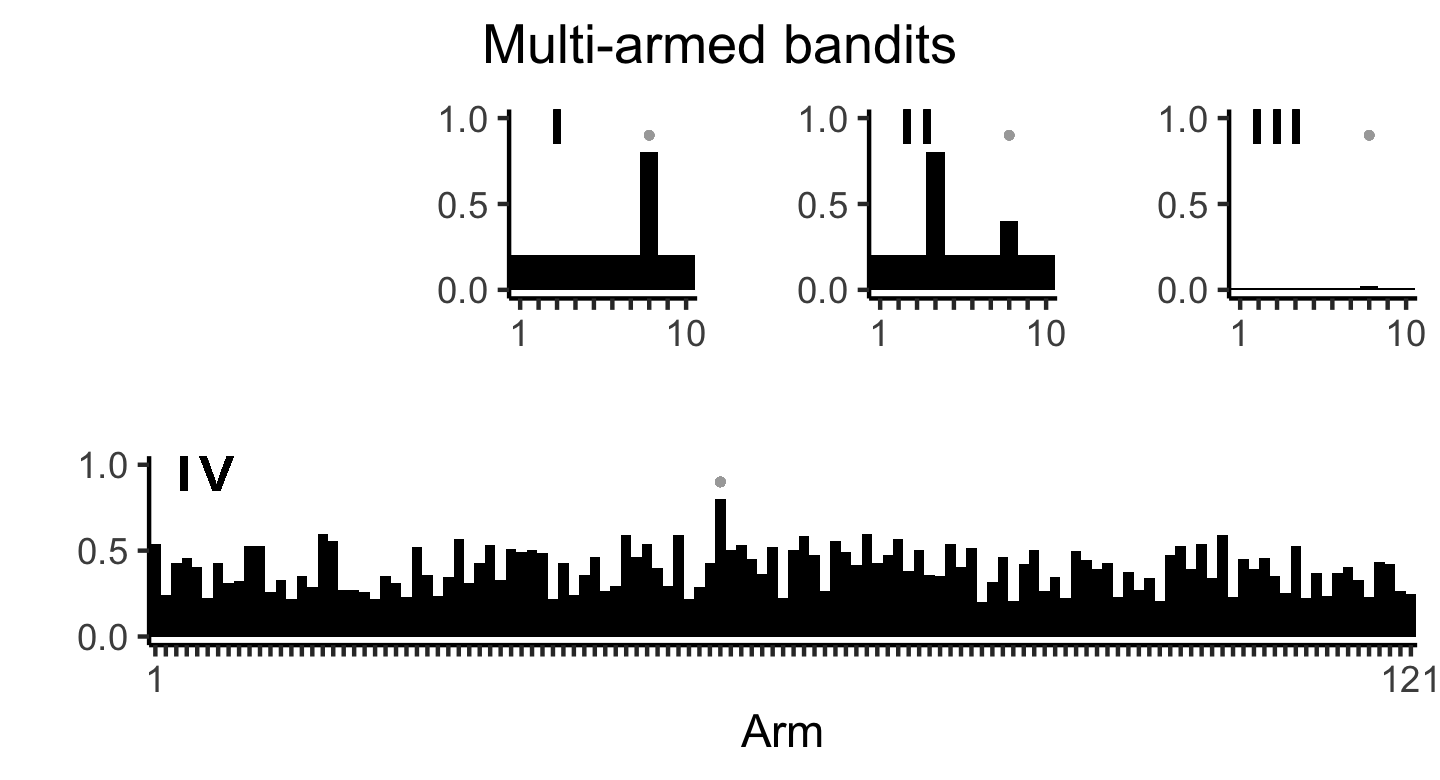
\includegraphics[width=.95\linewidth]{figures/fig2.png} 
	\caption{ \label{fig:f2} Bandits. Reward probabilities for each arm in bandit tasks I-IV. Grey dots highlight the optimal (i.e., highest reward probability) arm. See main text for a complete description.} 
\end{figure}

\begin{figure}
	[tbhp] \centering 
	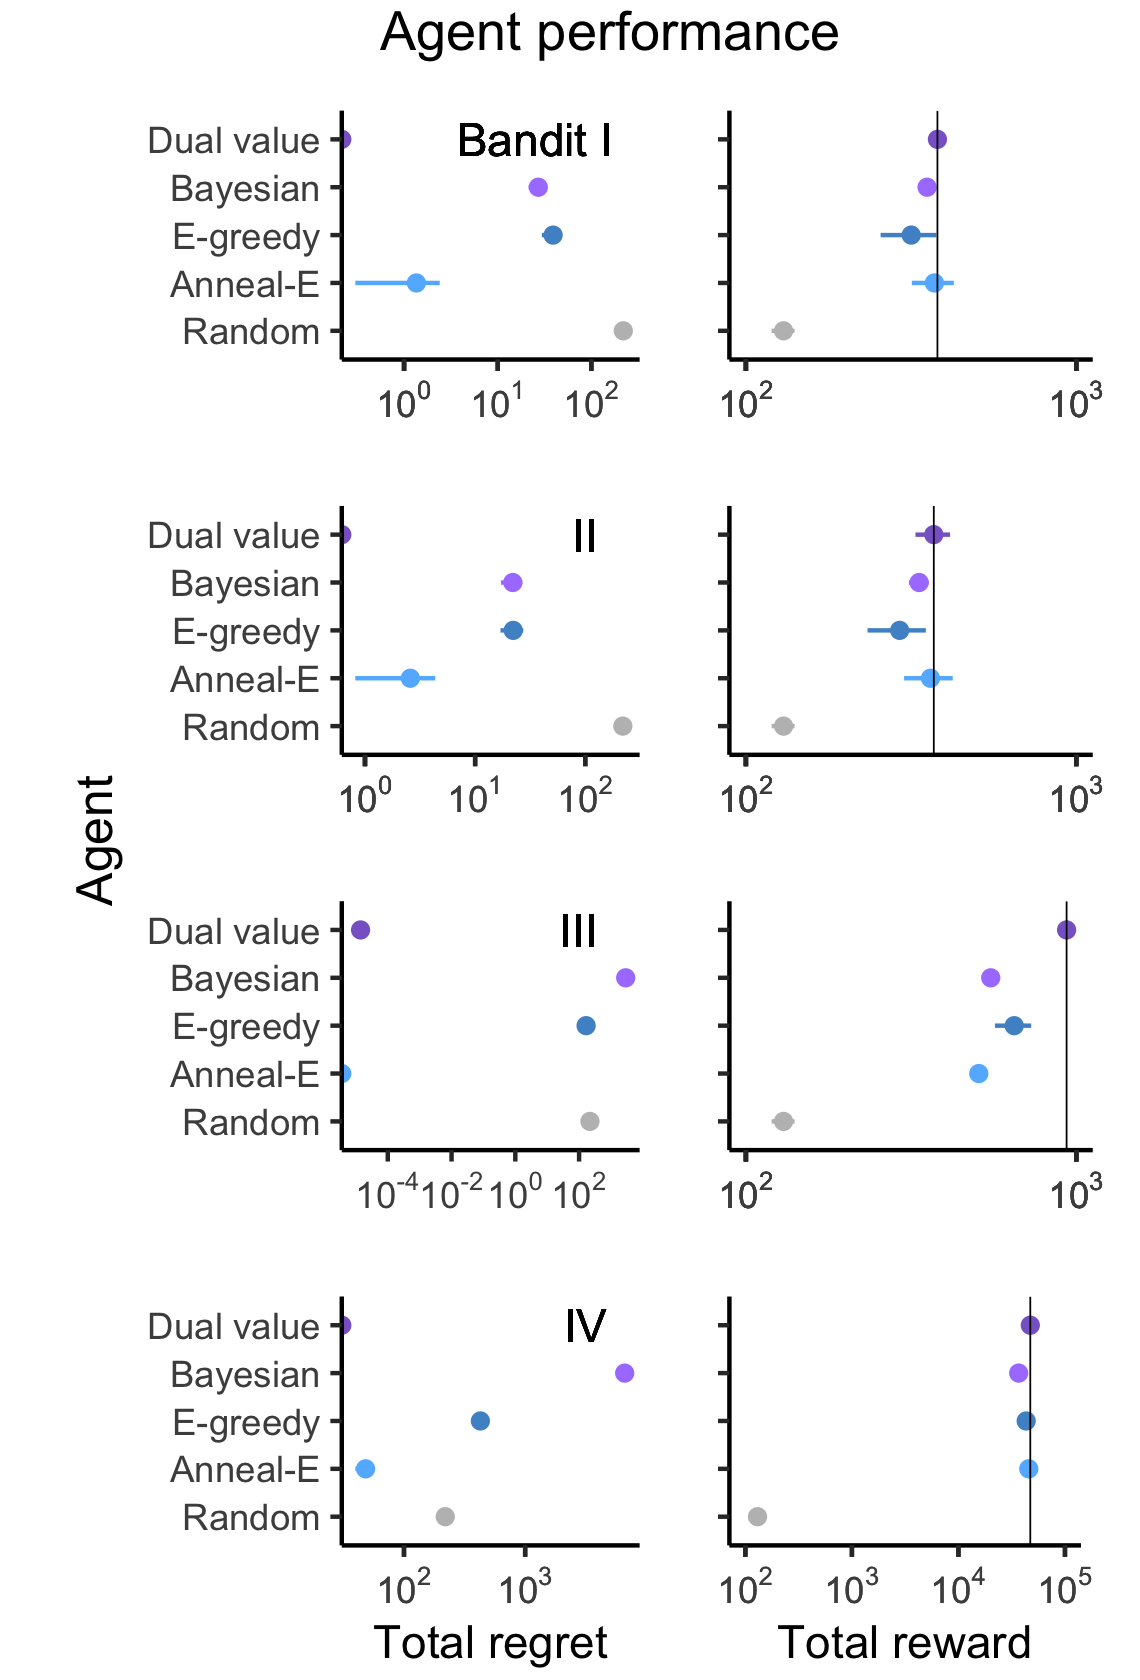
\includegraphics[width=.75\linewidth]{figures/fig3.png} 
	\caption{ \label{fig:f3} Regret and total accumulated reward across models and bandit task. Median total regret (left column) and median total reward (right column) for simulations of each model type ($N=100$ experiments per model). See main text and Table~\ref{tab:agents} for description of each model. Error bars in all plots represent median absolute deviation.} 
\end{figure}

To evaluate dual value learning (Eq.~\ref{eq:pipi}) we compared total reward and regret across a range of both simple, and challenging multi-armed bandit tasks. Despite its apparent simplicity, the essential aspects of the exploration-exploitation dilemma exist in the multi-armed bandit task \cite{Sutton2018}. Here the problem to be learned is the distribution of reward probabilities across arms (Figure ~\ref{fig:f2}).  To estimate the value of any observation $s_t$, we compare sequential changes in this probabilistic memory, $M_{t+dt}$ and $M_t$ using the KL divergence (i.e. relative entropy; Figure \ref{fig:supf1}\textbf{A}-\textbf{B}). The KL divergence is a standard way to measure the distance between two distributions \cite{MacKay2003} and is, by design, consistent with our axioms (see the \textit{Supplementary Materials} for a more thorough discussion). 

We start with a simple experiment involving a single high value arm. The rest of the arms have a uniform reward probability (Bandit \textbf{I}). This represents a trivial problem. Next we tried a basic exploration test (Bandit \textbf{II}), with one winning arm and one distractor arm whose value is close to but less than the optimal choice. We then move on to a more difficult sparse exploration problem (Bandit \textbf{III}), where the world has a single winning arm, but the overall probability of receiving any reward is very low ($p(R) = 0.02$ for the winning arm, $p(R) = 0.01$ for all others). Sparse reward problems are notoriously difficult to solve, and are a common feature of both the real world and artificial environments like Go, chess, and class Atari video games \cite{Mniha,Silver2016b,Silver2018}. Finally, we tested a complex, large world exploration problem (Bandit (\textbf{IV}) with 121 arms, and a complex, randomly generated reward structure. Bandits of this type and size are near the limit of human performance \cite{Wu2018}. 

We compared the reward and regret performance of 6 artificial agents. All agents used the same temporal difference learning algorithm (TD(0), \cite{Sutton2018}); see \textit{Supplementary materials}). The only difference between the agents was their exploration mechanism (Table~\ref{tab:agents}).  The e-greedy algorithm is a classic exploration mechanism \cite{Sutton2018}. Its annealed variant is common in state-of-the-art reinforcement learning papers, like Mnih \emph{et al} (\cite{Mniha}). Other state-of-the-art exploration methods are models that treat Bayesian information gain as an intrinsic reward and the goal of all exploration is to maximize total reward (extrinsic plus intrinsic) \cite{Jaegle2019,Schmidhuber1991}. To provide a lower bound benchmark of performance we included an agent with a purely random exploration policy.

\newcolumntype{L}{>{\arraybackslash}m{4cm}} 
\begin{table}[] 
    \centering 
	\caption{Artificial agents.} \label{tab:agents} 
	\begin{tabular}
		{|l|L|} \hline \textbf{Agent} & \textbf{Exploration mechanism} \\
		\hline Dual value & Our algorithm (Eq~\ref{eq:pipi}). \\
		\hline E-greedy & With probability $1-\epsilon$ follow a greedy policy. With probability $\epsilon$ follow a random policy. \\
		\hline Annealed e-greedy & Identical to E-greedy, but $\epsilon$ is decayed at fixed rate. \\
		\hline Bayesian reward & Use the KL divergence as a weighted intrinsic reward, sampling actions by a soft-max policy. $\sum_T R_t + \beta E_t$ \\
		\hline Random & Action are selected with a random policy (no learning) \\
		\hline 
	\end{tabular}
\end{table}

All of the classic and state-of-the-art algorithms performed well at the different tasks in terms of accumulation of rewards (right column, Figure \ref{fig:f3}). The one exception to this being the sparse low reward probability condition (Bandit \textbf{III}), where the dual value algorithm consistently returned more rewards than the other models. In contrast, most of the traditional models still had substantial amounts of regret in most of the tasks, with the exception of the annealed variant of the e-greedy algorithm during the sparse, low reward probability task (left column, Figure~\ref{fig:f3}). In contrast, the dual value learning algorithm consistently was able to maximize total reward with zero or near zero (Bandit \textbf{III}) regret, as would be expected by an optimal exploration policy.


\section*{Discussion}
\subsection*{Past work}
We are certainly not the first to quantify information value \cite{Kolchinsky2018,CogliatiDezza2017}, or use that value to optimize reward learning \cite{Kelly1956,Schmidhuber1991,Dayan1996,deAbril2018,Itti2009}. Information value though is typically framed as a means to maximize the amount of tangible rewards (e.g., food, water, money) accrued over time \cite{Sutton2018}. This means that information is treated as an analog of these tangible or external rewards (i.e., an \textit{intrinsic reward}) \cite{Schmidhuber1991,Berger-Tal2014,Itti2009,Friston2016}. This approximation does drive exploration in a practical and useful way, but doesn't change the intractability of the dilemma \cite{Thrun1992a,Dayan1996,Findling2018,Gershman2018b}. 

% Many accounts of information value rely on both Bayesian reasoning, and information theory \cite{Kelly1956,Itti2009,Friston2016}. In a formal, descriptive, or mathematical world, using these makes sense. However for a naturalistic theory of learning these are strong assumptions, that may not hold up. For example, if it turns out that animals are not in fact general Bayesian reasoning systems. 

At the other extreme from reinforcement learning are pure exploration methods, like curiosity \cite{Berlyne1950,Jaegle2019,Pathak2017} or PAC approaches \cite{Valiant1984}. Curiosity learning is not generally known to converge on rewarding actions with certainty, but never-the-less can be an effective heuristic \cite{Pathak2017,Burda2018,Colas2019}. Within some bounded error, PAC learning is certain to converge \cite{Valiant1984}. For example, it will find the most rewarding arm in a bandit, and do so with a bounded number of samples \cite{Even-Dar2002}. However, the number of samples is fixed and based on the size of the environment (but see \cite{Even-Dar2006,Strehl2009}). So while PAC will give the right answer, eventually, its exploration strategy also guarantees high regret.

% Cisek (2019) traced the evolution of perception, cognition, and action circuits from the Metazoan to the modern age \cite{Cisek2019}. The circuits for reward exploitation and observation-driven exploration appear to have evolved separately, and act competitively--exactly the model we suggest. In particular he notes that exploration circuits in early animals were closely tied to the primary sense organs (i.e. information) and, historically anyway, had no input from the homeostatic circuits needed for reward valuation \cite{Keramati2014,Cisek2019,Juechems2019}. 


\subsection*{Animal behavior}
In psychology and neuroscience, curiosity and reinforcement learning have developed as separate disciplines \cite{Berlyne1950,Kidd2015,Sutton2018}. And they are separate problems, with links to different basic needs: gathering resources to maintain physiological homeostasis \cite{Keramati2014,Juechems2019} and gathering information to plan for the future \cite{Valiant1984,Sutton2018}. Here we suggest that though they are separate problems, they are problems that can, in large part, solve one another.

The theoretical description of exploration in scientific settings is probabilistic \cite{Calhoun2014,Song2019a,Gershman2018b,Schulz2018a}. By definition probabilistic models can't make exact predictions of behavior, only statistical ones. Our approach is deterministic, and so does make exact predictions. Our theory predicts that it should be possible to guide exploration in real-time using, for example, optogenetic methods in neuroscience, or well timed stimulus manipulations in economics or other behavioral sciences. 

In species ranging from human to \textit{Caenorhabditis elegans}, there are hundreds perhaps thousands of exploration-exploitation experiments. Analysis of their behavior has been generally been limited to aggregate distributions. A deterministic theory can, in principle, open up entirely new avenues for reanalysis--using our model to make exact temporal predictions.

\subsection*{Exploration in the brain}
% TODO - some animals have exploration modules which seem to be orthoonal from reward.

\subsection*{Artificial intelligence}
Progress in reinforcement learning and artificial intelligence research is limited by three factors: data efficiency, exploration efficiency, and transfer learning \cite{Ha2018}. Our algorithm speaks directly to all three of these limits. 

In the large and complex environments that modern machine learning operates in random exploration takes too long to be practical. So there is a critical need for more efficient exploration strategies \cite{Ha2018}. These are often known as active sampling, or directed exploration. A range of heuristics for this kind of exploration have been explored \cite{Gottlieb2018,Epshteyn2008,Thrun1992b,Ishii2002a,Bellemare2016,Haarnoja2018}. But our dual value algorithm offers a principled approach. Designing efficient exploration reduces to two questions: what should our agent remember? How should we measure change change in that memory? This is subject to the axioms and Eq.~\ref{eq:pipi}, of course.

\subsection*{In the classroom}


\subsection*{Everyday life} The uncertainty of the unknown can always be recast as an opportunity to learn. But rather than being a trick of psychology, we prove this view is--in our formalism--mathematically optimal.


\subsection*{Acknowledgments.}
EP and TV wish to thank Jack Burgess, Matt Clapp, Kyle ``Donovank'' Dunovan, Richard Gao, Roberta Klatzky, Jayanth Koushik, Alp Muyesser, Jonathan Rubin, and Rachel Storer for their comments on earlier drafts. EP also wishes to thank Richard Grant for his illustration work in Figure 1.

The research was sponsored by the Air Force Research Laboratory (AFRL/AFOSR) award FA9550-18-1-0251. The views and conclusions contained in this document are those of the authors and should not be interpreted as representing the official policies, either expressed or implied, of the Army Research Laboratory or the U.S. government. TV was supported by the Pennsylvania Department of Health Formula Award SAP4100062201, and National Science Foundation CAREER Award 1351748.

\bibliography{library}

%%%%%%%%%%%%%%%%%%%%%%%%%%%%%%%%%%%%%%%%%%%%%%%%%%%%%%%%%%%%%%%%%%%%%%%%%%%%
% --------------------------------------------------------------------------
%%%%%%%%%%%%%%%%%%%%%%%%%%%%%%%%%%%%%%%%%%%%%%%%%%%%%%%%%%%%%%%%%%%%%%%%%%%%
\section*{Supplementary materials.}

\subsection*{Dual value implementation}
\subsubsection*{Value initialization and tie breaking} \label{sec:init_ties}
The initial value $E_0$ for $\pi^*_E$ can be arbitrary, with the limit $E_0 > 0$. In theory $E_0$ does not change $\pi^*_E$'s long term behavior, but different values will change the algorithm's short-term dynamics and so might be quite important in practice. By definition a pure greedy policy, like $\pi^*_E$, cannot handle ties. There is simply no mathematical way to rank equal values. Theorems~\ref{theorem:convergence} and~\ref{theorem:Z} ensure that any tie breaking strategy is valid, however, like the choice of $E_0$, tie breaking can strongly affect the transient dynamics. Viable tie breaking strategies taken from experimental work include, ``take the closest option'', ``repeat the last option'', or ``take the option with the highest marginal likelihood''. We do suggest the tie breaking scheme is deterministic, which maintains the determinism of the whole theory. See \emph{Information value learning} section below for concrete examples both these choices.

\subsubsection*{The rates of exploration and exploitation}
In Theorem~\ref{theorem:meta} we proved that $\pi_{\pi}$ inherits the optimality of policies for both exploration $\pi_E$ and exploitation $\pi_R$ over infinite time. However this does proof does not say whether $\pi_{\pi}$ will not alter the rate of convergence of each policy. By design, it does alter the rate of each, favoring $\pi_R$. As you can see in Eq.~\ref{eq:meta_greedy}, whenever $r_t = 1$ then $\pi_R$ dominates that turn. Therefore the more likely $p(r=1)$, the more likely $\pi_R$ will have control. This doesn't of course change the eventual convergence of $\pi_E$, just delays it in direct proportion to the average rate of reward. In total, these dynamics mean that in the common case where rewards are sparse but reliable, exploration is favored and can converge more quickly. As exploration converges, so does the optimal solution to maximizing rewards.

\subsubsection*{Re-exploration}
The world often changes. Or in formal parlance, the world is non-stationary process. When the world does change, re-exploration becomes necessary. Tuning the size of $\epsilon$ in $\pi_{\pi}$ (Eq~\ref{eq:meta_greedy}) tunes the threshold for re-exploration. That is, once the $\pi^*_E$ has converged and so $\pi^*_R$ fully dominates $\pi_{\pi}$, if $\epsilon$ is small then small changes in the world will allow $pi_E$ to exert control. If instead $\epsilon$ is large, then large changes in the world are needed. That is, $\epsilon$ acts a hyper-parameter controlling how quickly rewarding behavior will dominate, and easy it is to let exploratory behavior resurface.


\subsection*{Bandits}
\subsubsection*{Design} Like the slot machines which inspired them, each bandit returns a reward according to a predetermined probability. As an agent can only chose one bandit (``arm'') at a time, so it must decide whether to explore and exploit with each trial.

We study four prototypical bandits. The first has a single winning arm ($p(R) = 0.8$, Figure \ref{fig:f2}\textbf{A}); denoted as bandit \textbf{I}. We expect any learning agent to be able to consistently solve this task. Bandit \textbf{II} has two winning arms. One of these (arm 7, $p(R) = 0.8$) though higher payout than the other (arm 3, $p(R) = 0.6$). The second arm can act as a ``distractor'' leading an to settle on this suboptimal choice. Bandit \textbf{III} also has a single winning arm, but the overall probability of receiving any reward is very low ($p(R) = 0.02$ for the winning arm, $p(R) = 0.01$ for all others). Sparse rewards problems like these are difficult to solve and are common feature of both the real world, and artificial environments like Go, chess, and class Atari video games \cite{Mniha,Silver2016b,Silver2018}. The fourth bandit (\textbf{IV}) has 121 arms, and a complex randomly generated reward structure. Bandits of this type and size are probably at the limit of human performance \cite{Wu2018}. 

\subsubsection*{World model and distance}
All bandits share a simple basic common structure. The have a set of $n$-arms, each of which delivers rewards in a probabilistic fashion. This lends itself to simple discrete n-dimensional world model, with a memory  slot for each arm/dimension. Each slot then represents the independent probability of receiving a reward (Supp. Fig~\ref{fig:supf1}\textbf{A}). 

The Kullback--Leibler divergence (KL) is a widely used information theory metric, which measures the information gained by replacing one distribution with another. It is highly versatile and widely used in machine learning \cite{Goodfellow-et-al-2016}, Bayesian reasoning \cite{Itti2009,Friston2016}, visual neuroscience \cite{Itti2009}, experimental design \cite{Lopez-Fidalgo2007}, compression \cite{Mackay,Still2012} and information geometry \cite{Ay2015}, to name a few examples. KL has seen extensive use in reinforcement learning. % Cites

The Kullback--Leibler ($KL$) divergence satisfies all five value axioms (Eq.~\ref{eq:KL}). 

Itti and Baladi \citep{Itti2009} developed an approach similar to ours for visual attention, where our information value is identical to their \textit{Bayesian surprise}. Itti and Baladi (2009) showed that compared to range of other theoretical alternative, information value most strongly correlates with eye movements made when humans look at natural images. Again in a Bayesian context, KL plays a key role in guiding \textit{active inference}, a mode of theory where the dogmatic central aim of neural systems is make decisions which minimize free energy \cite{Friston2016,Schwartenbeck2019}. 

\begin{definition}
    Let $E$ represent value of information, such that $E := KL(M_{t+dt}, M_t)$ (Eq.~\ref{eq:KL}) after observing some state $s$.
\end{definition}

\begin{equation}
    KL(M_{t+dt}, M_t) = \sum_{s \in S} M_{t+dt}(s) \text{log} \frac{M_{t+dt}(s)}{M_t(s)} 
    \label{eq:KL}
\end{equation}

Axiom~\ref{ax:1} is satisfied by limiting $E$ calculations to successive memories. Axiom~\ref{ax:2}-\ref{ax:3} are naturally satisfied by KL. That is, $E = 0$ if and only if $M_{t+dt} = M_t$ and $E \geq 0$ for all pairs $(M_{t+dt}, M_t)$.

To make Axiom~\ref{ax:5} more concrete, in Figure~\ref{fig:supf2} we show how KL changes between a hypothetical initial distribution (always shown in grey) and a ``learned'' distribution (colored). For simplicity's sake we use a simple discrete distribution representing a 10-armed bandit, though the illustrated patterns hold true for any pair of appropriate distributions. In Figure~\ref{fig:supf2}\textbf{C} we see KL increases substantially more for a local exchange of probability compared to an even global re-normalization (compare panels \textit{A.} and \textit{B.}). 

\begin{figure}
	[tbhp] \centering 
	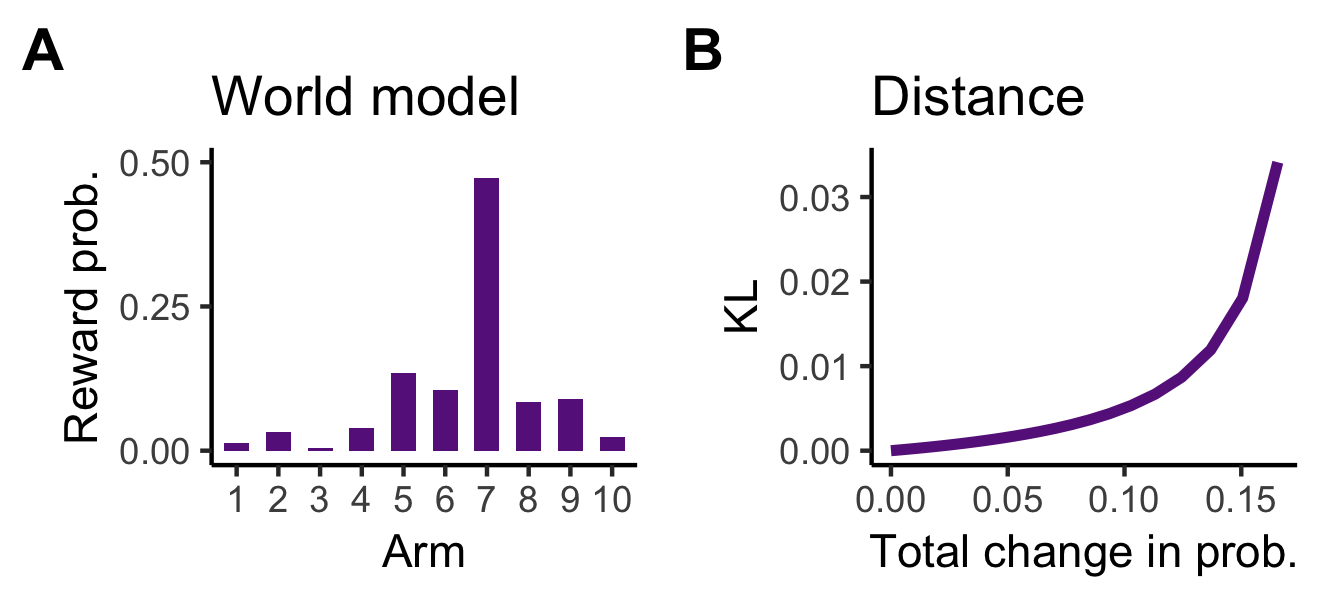
\includegraphics[width=.95\linewidth]{figures/subfig1.png} 
	\caption{\label{fig:supf1} A world model for bandits.
	\textbf{B}. Example of a single world model suitable for all bandit learning.
	\textbf{B} Changes in the KL divergence--our choice for the distance metric during bandit learning--compared to changes in world model, as by measured the total change in probability mass.}
\end{figure}

\begin{figure}
	[tbhp] \centering 
	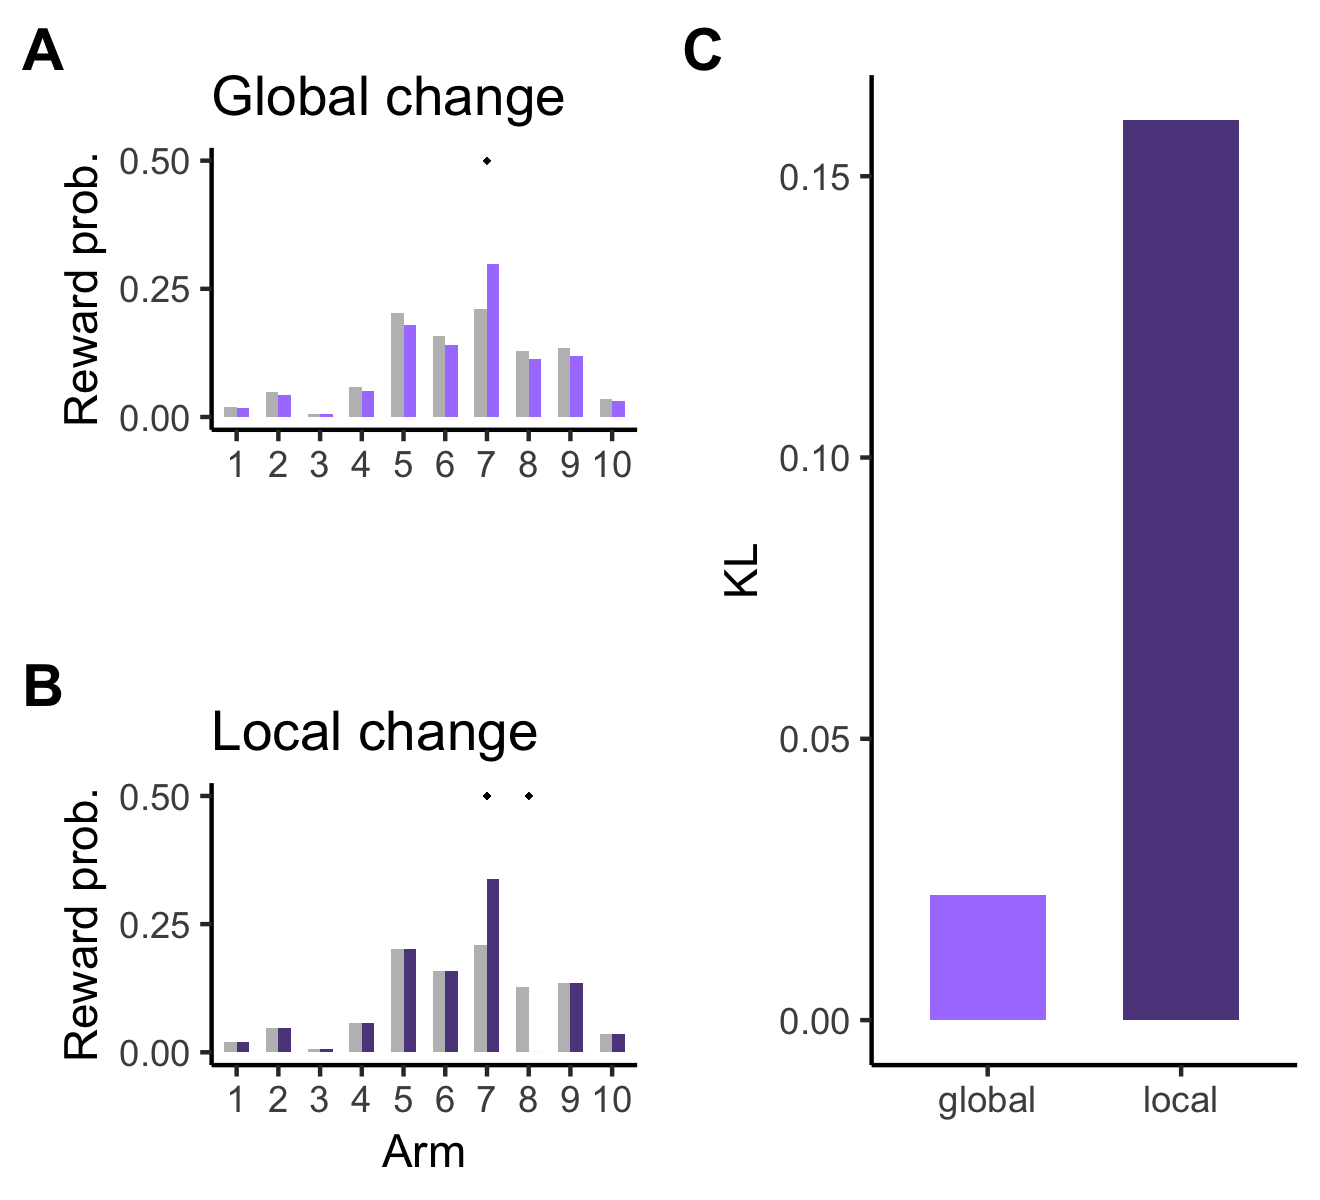
\includegraphics[width=.95\linewidth]{figures/subfig2.png} 
	\caption{\label{fig:supf2} An example of observation specificity during bandit learning. 
	\textbf{A}. A initial (grey) and learned (distribution), where the hypothetical observation $s$ increases the probability of arm 7 by about 0.1, and the expense of all the other probabilities.
	\textbf{B}. Same as A except that the decrease in probability comes only from arm 8.
	\textbf{C}. The KL divergence for local versus global learning.
	}
\end{figure}

\subsubsection*{Initializing $\pi_\pi$}
In these simulations we assume that at the start of learning an animal should have a uniform prior over the possible actions $A \in \mathbb{R}^K$. Thus $p(a_k) = 1/K$ for all $a_k \in A$. We transform this uniform prior into the appropriate units for our KL-based $E$ using Shannon entropy, $E_0 = \sum_K p(a_k)\ \text{log}\ p(a_k)$. 

In our simulations we use a tie breaking ``right next'' heuristic which keeps track of past breaks, and in a round robin fashion iterates rightward over the action space.

\subsubsection*{Reinforcement learning} Reinforcement learning in all agent models was done with using the TD(0) learning rule \cite{Sutton2018} (Eq. \ref{eq:TD}). Where $V(s)$ is the value for each state (arm), $\mathbf{R}_t$ is the \emph{return} for the current trial, and $\alpha$ is the learning rate $(0-1]$. See the \emph{Hyperparameter optimization} section for information on how $\alpha$ chosen for each agent and bandit.

\begin{equation}
	\label{eq:TD}
	V(s) = V(s) + \alpha (\mathbf{R}_t - V(s)
\end{equation}

The return $\mathbf{R}_t$ differed between agents. Our dual value agent, and both the variations of the e-greedy algorithm, used the reward from the environment $R_t$ as the return. This value was binary. The Bayesian reward agent used a combination of information value and reward $\mathbf{R}_t = R_t + \beta E_t$, with the weight $\beta$ tuned as described below. 

\subsubsection*{Hyperparameter optimization}
The hyperparameters for each agent were tuned independently for each bandit using a modified version of Hyperband \cite{Li2016a}. For a description of hyperparameters seen Table \ref{tab:agents}, and for the values themselves Table~\ref{table:hp}.

\begin{table}[]
\caption{Hyperparameters for individual bandits (\textbf{I}-\textbf{IV}).}
\label{tab:hp}
\begin{tabular}{|l|l|l|l|l|l|}
\hline
\textbf{Agent} & \textbf{Parameter} & \textbf{I} & \textbf{II} & \textbf{III} & \textbf{IV} \\ \hline
Dual value & $\eta$ & 0.053 & 0.017 & 0.003 & 5.8e-09 \\ \hline
Dual value & $\alpha$ & 0.34 & 0.17 & 0.15 & 0.0011 \\ \hline
E-greedy & $\epsilon$ & 0.14 & 0.039 & 0.12 & 0.41 \\ \hline
E-greedy & $\alpha$ & 0.087 & 0.086 & 0.14 & 0.00048 \\ \hline
Annealed e-greedy & $\tau_E$ & 0.061 & 0.084 & 0.0078 & 0.072 \\ \hline
Annealed e-greedy & $\epsilon$ & 0.45 & 0.98 & 0.85 & 0.51 \\ \hline
Annealed e-greedy & $\alpha$ & 0.14 & 0.19 & 0.173 & 0.00027 \\ \hline
Bayesian & $\beta$ & 0.066 & 0.13 & 0.13 & 2.14 \\ \hline
Bayesian & $\alpha$ & 0.066 & 0.03 & 0.17 & 0.13 \\ \hline
Bayesian & $\gamma$ & 0.13 & 0.98 & 0.081 & 5.045 \\ \hline
\end{tabular}
\end{table}

\subsubsection*{Exploration and value dynamics}. 
While agents earned nearly equivalent total reward in Bandit I (Fig~\ref{fig:f3}, \textit{top row}), their exploration strategies were quite distinct. In Supp. Fig~\ref{fig:supf3}\textbf{B}-\textbf{D}) we compare three prototypical examples of exploration, for each major class of agent: ours, Bayesian, and E-greedy for Bandit \textit{I}. In Supp. Fig~\ref{fig:supf3}\textbf{A}) we include an example of value learning value learning in our agent.

\begin{figure}
	[tbhp] \centering 
	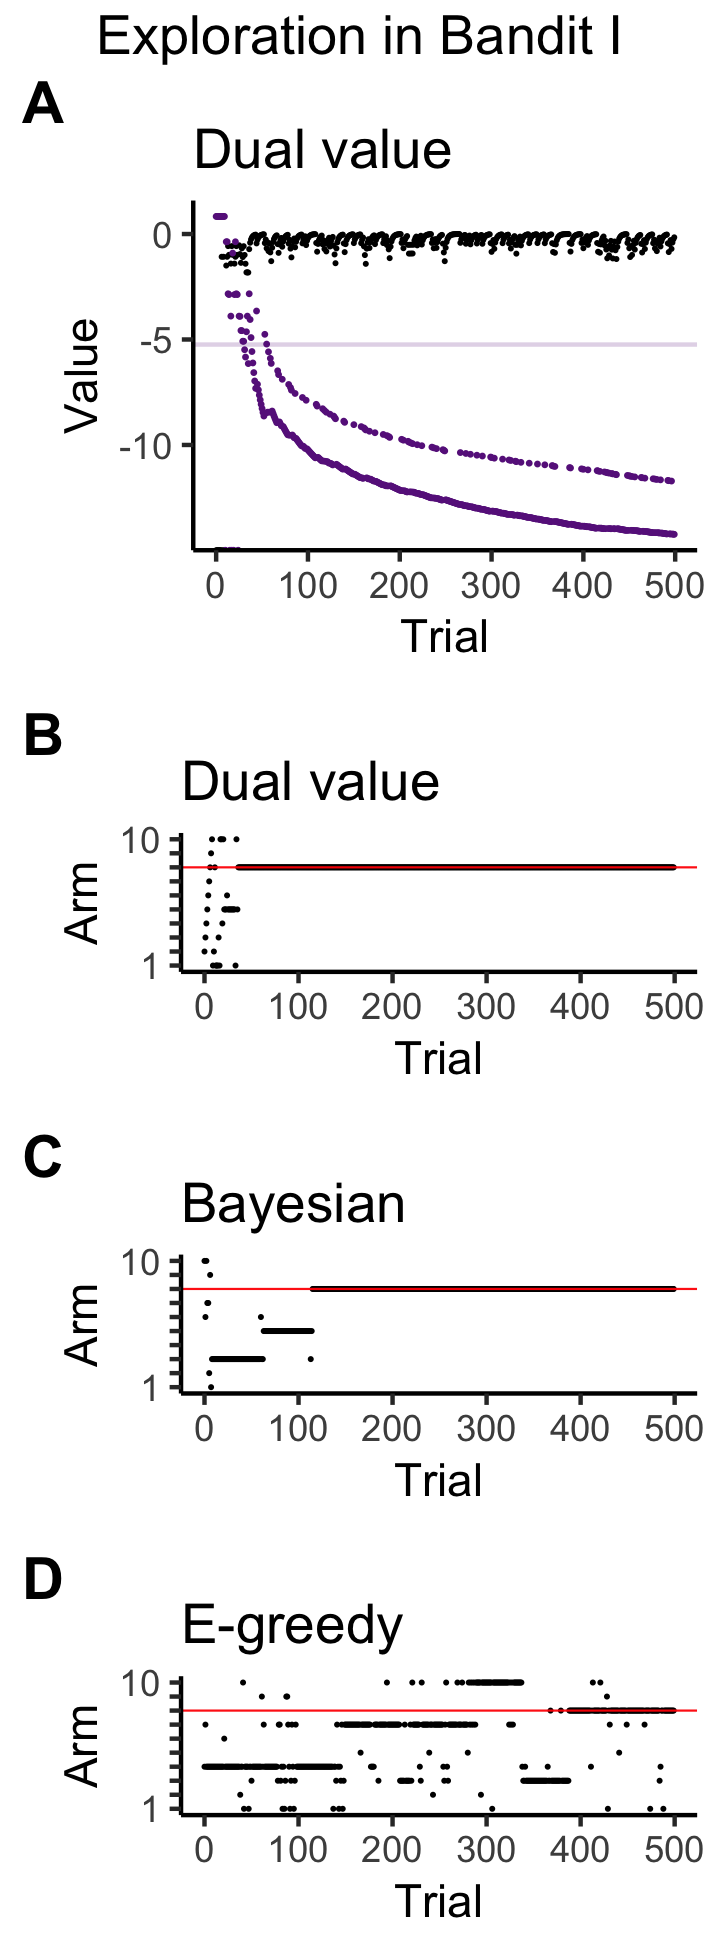
\includegraphics[width=.5\linewidth]{figures/subfig3.png} 
	\caption{\label{fig:supf3} Exploration and value dynamics.
	\textbf{A}. An example of our dual value learning algorithm during 500 trials on Bandit. The light purple line represents the boredom threshold $\eta$ (Eq.~\ref{eq:pipi}).
	\textbf{B.} An example of exploration dynamics (i.e arm selection) on Bandit. Note how the search is structured, and initially sequential.  
	\textbf{C-D.} Exploration dynamics for two other agents. \textbf{C.} The Bayesian agent, which like our algorithm uses active sampling, and values information. Note how this shows a mixture of structures and repeated choices, mixed with seemingly random behavior. \textbf{D.} The E-greedy agent, which uses purely random sampling. Note how here the agent is either greedy, repeating the same arm, or seemingly random.}
\end{figure}

\section*{Mathematical Appendix.}
\newcommand{\beginsupplement}{%
        \setcounter{table}{0}
        \renewcommand{\thetable}{S\arabic{table}}%
        \setcounter{figure}{0}
        \renewcommand{\thefigure}{S\arabic{figure}}%
     }
\beginsupplement
\setcounter{theorem}{0}

% --------------------------------------------------------------------------
\subsection*{Optimal substructure in memory}
To find an optimal value solution for $\hat E$ using the Bellman equation we must prove our memory $\mathbf{M}$ has optimal substructure. This is because the normal route, which assumes the problem rests in a Markov Space, is closed to us. By optimal substructure we mean that the process of learning in $\mathbf{M}$, and therefore maximization of $\hat E$ can be partitioned into a collection, or series of memories, each of which is itself an max value solution.

This opaque term of optimal substructure can be intuitivily understood by looking in turn at another theoretical construct, Markov spaces. 

In Markov spaces there are a set of states $(S_0, S_1, \ldots)$, where the transition to the next $S_t$ depends only on the previous state $S_{t-1}$. This limit means that if we were to optimize over these states, as in reinforcement learning, we know that we can treat each transition as its own ``subproblem'', and ignore the history's $(S_0, S_1, \ldots)$ effect on value, and therefore the overall situation has ``optimal substructure''.

The problem for our defintion of information value is it relies on memory which is necessarily composed of many past observations, in many orders, and so it cannot be a Markov space. So if we wish to use the Bellman equation, we need to find another way to establish optimal substructure. This is the focus of Theorem~\ref{theorem:opt_sub}. In this theorem we implicitly assume that $\mathbf{X} = \mathbf{S}$, $\mathbf{A}$, $\mathbf{M}$, $f$, and $\Lambda$ are given, and that $\Lambda$ is deterministic, 

\begin{theorem}[Optimal substructure] \label{theorem:opt_sub} 
   If $V^*_{\pi_{\hat E}}$ is the optimal information value given by policy $\pi_{\hat E}$, a memory $\mathbf{M}_t$ has optimal substructure if the last observation $X$ can be removed from $\mathbf{M}$, by $\mathbf{M-1}_{t} = f^{-1}(\mathbf{X}, \mathbf{M}_t)$ such that the resulting value $V^*_{t-1} = V^*_{t} - E_{t}$ is also optimal. 
\end{theorem}
\begin{proof}
	Given a known optimal value $V^*$ given by $\pi_{\hat E}$ we assume for the sake of contradiction there also exists an alternative policy $\hat \pi_{\hat E} \neq \pi_{\hat E}$ that gives a memory $\hat{\mathbf{M}}_{t-1} \neq \mathbf{M}_{t-1}$ and for which $\hat V^*_{t-1} > V^*_{t-1}$. 
	
	To recover the known optimal memory $\mathbf{M}_t$ we lift $\hat{\mathbf{M}}_{t-1}$ to $\mathbf{M}_t = f(\hat{\mathbf{M}}_{t-1}, \mathbf{X}_t)$. This implies $\hat V^* > V^*$ which in turn contradicts the purported original optimality of $V^*$ and therefore $\hat \pi_{\hat E}$.
\end{proof}

This proof requires two things. First, we need to a mechanism of forgetting, of a very particular kind. We assume that the last learning step $f(\mathbf{X}, \mathbf{M}) \rightarrow \mathbf{M}'$ can be undone by a new vector valued function $f^{-1}$, such that $f(\mathbf{X}, \mathbf{M'}) \rightarrow \mathbf{M}$. In other words we must assume what was last remembered, can always be exactly forgotten. Second, we assume the environmental dynamics, given by the transition function $\Lambda$, are deterministic. 

Determinism is consistent with the natural world which does evolve in a deterministic way, at the scale of animal behavoir that we concerned with at least. This assumption is however at odds with much of reinforcement learning theory \cite{Sutton2018} and past experimental work. For example, \cite{Gershman2018}. Both tend to study stochastic environments. We addressed this discrepancy in the main text, using numerical simulations.


% ------------------------------------------------------------------------
\subsection*{Bellman optimal information collection}
We aim to find a series of actions $(\mathbf{A}_1, \mathbf{A}_2, ..\mathbf{A}_T)$, drawn from a set $\mathbb{A}$, that maximize each payout $(\hat E_0, \hat E_1, \ldots, \hat E_{T})$ so the total payout received is as large as possible. If there is a policy $\mathbf{A} = \pi(\mathbf{X})$ to take actions, based on a series of observations $(X_0, X_1, ..X_{T}),$, given by $\Lambda$, then an optimal policy $\pi^*$ will always find the maximum total value $V^* = \argmax_{\mathbf{A} \in \mathbb{A}} \sum_T \hat E_t $. In the form above one would need to reconsider the entire sequence of actions for any one change to that sequence, leading to a combinatorial explosion. Bellman's insight was a way to make this last problem simpler by breaking it down into a small set of subproblems that we can solve in a tractable way without an explosion in complexity. This is his principle of optimality, which reads:

\begin{quote}
    An optimal policy has the property that whatever the initial state and initial decision are, the remaining decisions must constitute an optimal policy with regard to the state resulting from the first decision. \cite{Bellmann1954}
\end{quote}

Mathematically Bellman's principle allows us to translate the full problem, $V^* = \argmax_{\pi} \sum_T \hat E_1, \hat E_2, ..., \hat E_{T}$ to a recursive one. Having already proven the optimal substructure of $\mathbf{M}$, and given an arbitrary starting value $E_0$, the Bellman solution to curiosity optimization of $\hat E$ is therefore given by,

\begin{equation} 
	\label{eq:bellman_iter_E_app}
	V^*_{\hat E}(\mathbf{S}) = \argmax_{\mathbf{A} \in \mathbb{A}} \Big [ \hat E_{t}  + V^*_{\hat E}(\Lambda(\mathbf{S},\mathbf{A})) \Big ]
\end{equation}


% ------------------------------------------------------------------------
\subsection*{Optimal exploration} 

Recall from the main text we consider that a good exploration should,

\begin{enumerate}
	\item Exploration should visit all available states of the environment at least once.
	\item Exploration should cease when learning has plateaued.
	\item Exploration should take as few steps as possible to achieve 1 and 2.
\end{enumerate}

If $\pi_{\hat E}$ to a deterministic policy this makes proving these three properties amounts to solving sorting problems on $\hat E$, and assuming $\mathbf{X} = \mathbf{S}$. That is, if a state is visited by our algorithm it must have the highest value, by definition. So if every state must be visited every state must, at one time or another, give the maximum value. This is certain to happend if we know that all values will begin contracting towards zero, in finite time. 

\textbf{Definitions.} Let $\mathbb{Z}$ be the set of all visited states, where $\mathbb{Z}_0$ is the empty set $\{\}$ and $\mathbb{Z}$ is built iteratively over a path $P$, such that $\mathbb{Z} \rightarrow \{\mathbf{S} | \mathbf{S} \in \mathbb{S}\ \text{and}\ x \not\in \mathbf{Z}\}$. 

To formalize the idea of ranking we take an algebraic approach. Give any three real numbers $(a,b,c)$,

\begin{align}\label{eq:ineq} 
	a \leq b \Leftrightarrow \exists \ c;\ b = a + c \\
	a > b \Leftrightarrow (a \neq b) \wedge (b \leq a) 
\end{align}

\begin{theorem}[Complete exploration] \label{theorem:Z} 
	Given some arbitrary value $\hat E_0$, an exploration policy governed by $\pi_{\hat E}$ will visit all states $\mathbf{S} \in \mathbb{S}$ in finite number of steps $T$.
\end{theorem}
\begin{proof}
	Let $\mathbf{E} = (\hat E_1, \hat E_2, ...)$ be ranked series of $\hat E$ values for all states $\mathbf{S}$, such that $(\hat E_1 \geq \hat E_2, \geq ...)$. To swap any pair of values ($\hat E_i \geq \hat E_j$) so ($\hat E_i \leq \hat E_j$) by Eq.~\ref{eq:ineq} $\hat E_i - c = \hat E_j$. 
	
	Therefore, again by Eq.~\ref{eq:ineq}, $\exists \int \delta \hat E \rightarrow -c$. 
	
	\textit{Recall}: Axiom 4 - $\nabla^2 \mathbf{M} < 0$ after a finite time $T^*$.
	
	However if we wished to instead swap ($\hat E_i \leq \hat E_j$) so ($\hat E_i \geq \hat E_j$) by definition $\not \exists c; \hat E_i + c = \hat E_j$, as $\not \exists \int \delta \hat E \rightarrow c$. 
	
	To complete the proof, assume that some policy $\hat \pi_{\hat E} \neq \pi^*_E$. By definition policy $\hat \pi_{\hat E}$ can be any action but the maximum, leaving $k-1$ options. Eventually as $t \rightarrow T*$ the only possible swap is between the max option and the $kth$, but as we have already proven this is impossible as long as Axiom 4 holds. Therefore, the policy $\hat \pi_{\hat E}$ will leave at least 1 option unexplored and $S \neq Z$. 
\end{proof}

\begin{theorem}[[Efficient exploration] \label{theorem:convergence} 
	An exploration policy governed by $\pi^*_{\hat E}$ will revisit all states in exact proption to their information value.
\end{theorem}
\begin{proof}
    \textit{Recall}: Theorem~\ref{theorem:Z}.
    \textit{Recall}: $\pi^*_E$ is a maximum value deterministic algorithm.
	\textit{Recall}: Axiom 2. Each time $\pi^*_E$ visits a state $\mathbf{S}$, so $\mathbf{M} \rightarrow \mathbf{M}'$, and after $T^*$ it is axiomatically true $\hat{E}' < \hat E$
	
	By induction then, if $\pi^*E$ will visit all $\mathbf{S} \in \mathbb{S}$ in $T^*$ trials, it will revisit them at most $2T^*$, therefore as $t \rightarrow \infty$, $E \rightarrow \eta$, where $eta > 0$. 
\end{proof}

These exploration proofs come with some fine print, for practical work. $E_0$ can be any positive and finite real number, $E_0 > 0$. Different choices for $E_0$ will not change the proofs, especially their convergence. So in that sense one can chosen it in an arbitrary way. Different choices for $E_0$ can however change individual choices, and their order. This can be quite important in practice, especially when trying to describe some real data.  

% ---------------------------------------------------------------------------------
\subsection*{Optimality of $\Pi_{\pi}$} 
Recall that in the main text we introduce the equation below as a candidate with zero regret solution to exploration-exploitation problems, set in terms the mixed value sequence $V_{\hat{E}R}$.

\begin{equation} 
    \label{eq:pipi_app}
    \begin{split}
        \Pi_{\pi} = 
        \begin{cases}
            \pi^*_{\hat{E}} & : \hat{E} - \eta > R + \rho \\
            \pi_R 	& : \hat{E} - \eta < R + \rho \\
        \end{cases}
    \end{split}
\end{equation}

In the following section we prove two things about the optimality of $\pi_\pi$. First, if $\pi_R$ had any optimal asymptotic property for value learning before their inclusion into our scheduler, they retain that optimal property under $\pi_\pi$ when $\eta = 0$, or is otherwise sufficiently small. Second, show that if both $\pi_R$ and $\pi_E$ are greedy, and $\pi_\pi$ is greedy in its definition, then Eq~\ref{eq:pipi} is certain to maximize total value. The total value of $R$ and $\hat E$ is the exact quantity to maximize if information seeking and reward seeking are equally important, overall. This is, as the reader may recall, one of our key assumptions. Proving this optimality is analogous to the classic activity selection problem from the job scheduling literature \cite{BellmanBook,Roughgarden2019}.

\begin{theorem}[$\pi_{\pi}$ is unbiased] \label{theorem:meta} 
	 Let any $S$, $\mathbf{A}$, $\mathbf{M}$, $\pi_R$, $\pi_E$, and $\delta$ be given. Assuming an infinite time horizon, if $\pi_E$ is optimal and $\pi_R$ is optimal, then $\pi_{\pi}$ is also optimal in the same sense as $\pi_E$ and $\pi_R$. 
\end{theorem}
\begin{proof}
	The optimality of $\pi_{\pi}$ can be seen by direct inspection. If $p(R = 0) > 0$ we are given an infinite horizon, then $\pi_E$ will have a unbounded number of trials meaning the optimally of $P^*$ holds. Likewise, $\sum E < \eta$ as $T \rightarrow \infty$, ensuring $pi_R$ will dominate $\pi_{\pi}$ therefore $\pi_R$ will asymptotically converge to optimal behavior. 
\end{proof}

In proving this optimality of $\pi_{\pi}$ we limit the probability of a positive reward to less than one, denoted by $p(R_t = 1) < 1$. Without this constraint the reward policy $\pi_R$ would always dominate $\pi_{\pi}$ when rewards are certain. While this might be useful in some circumstances, from the point of view $\pi_E$ it is extremely suboptimal. The model would never explore. Limiting $p(R_t = 1) < 1$ is a reasonable constraint, as rewards in the real world are rarely certain. A more naturalistic way to handle this edge case is to introduce reward satiety, or a model physiological homeostasis \cite{Keramati2014,Juechems2019}.

In classic scheduling problems the value of any job is known ahead of time \cite{Bellmann1954,Roughgarden2019}. In our setting, this is not true. Reward value is generated by the environment, \textit{after} taking an action. In a similar vein, information value can only be calculated \textit{after} observing a new state. Yet Eq.~\ref{eq:pipi} must make decisions \textit{before} taking an action. If we had a perfect model of the environment, then we could predict these future values accurately with model-based control. In the general case though we don't know what environment to expect, let alone having a perfect model of it. As a result, we make a worst-case assumption: the environment can arbitrarily change--bifurcate--at any time. This is a highly nonlinear dynamical system \cite{Strogatz1994}. In such systems, myopic control--using only the most recent value to predict the next value-- is known to be an robust and efficient form of control \cite{Hocker2019}. We therefore assume that last value is the best predictor of the next value, and use this assumption along with Theorem~\ref{theorem:meta} to complete a trivial proof that Eq.~\ref{eq:pipi} maximizes total value.

\subsubsection*{A win-stay, lose-switch solution}
If we prove $\pi_{\pi}$ has optimal substructure, then using the same replacement argument \cite{Roughgarden2019} as in Theorem~\ref{theorem:meta}, a greedy policy for $\pi_\pi$ will maximize total value.

\begin{theorem}[No regret - mixed values]
	\label{th:no_regret_ER}
	When either $\pi_{\hat E}$ or $\pi_R$ is in control under $\Pi_{\pi}$, all actions are zero regret in terms of $V_{\hat{E}R}$. That is, $\sum_{k=0}^{T} G = 0$.
\end{theorem}

% HERE- TODO - this should be a simple substitution proof.

% \begin{theorem}[Total value maximization of $\pi_{\pi}$] \label{theorem:metA_total} 
%     \label{theorem:meta} 
% 	 Let any $S$, $A$, $\mathbf{M}$, $\pi_R$, and $\delta$ be given. If $\pi_R$ is defined on a Markov Decisions, then $\pi_\pi$ is Bellman optimal and will maximize total value. 
% \end{theorem}
% \begin{proof}
%     We assume Reinforcement learning algorithms are embedded in Markov Decisions space, which by definition has the same decomposition properties as that found in optimal substructure.
    
%     \textit{Recall}: The memory $\mathbf{M}$ has optimal substructure (Theorem~\ref{theorem:opt_sub}.
    
% 	\textit{Recall}: The asymptotic behavior of $\pi_R$ and $\pi_E$ are independent under $\pi_\pi$ (Theorem~\ref{theorem:meta}
	
% 	\textit{Recall}: The controller $\Pi_\pi$ is deterministic.
	
% 	If both $\pi_R$ and $\pi_E$ have optimal substructure independently, and are independent under $\Pi_\pi$, then $\Pi_\pi$ must also have optimal substructure. If $\pi_\pi$ has optimal substructure, then it is Bellman optimal.
% \end{proof}
 

\end{document} 
\bibliography{sample}
